% Slides accompanying "Learn RISC-V CPU Implementation and BSV" book
% Copyright (c) 2024 Rishiyur S. Nikhil, All Rights Reserved

% -*- mode: fundamental -*-

% Slides accompanying "Learn RISC-V CPU Implementation and BSV" book
% Copyright (c) 2024 Rishiyur S. Nikhil, All Rights Reserved

% This is a preamble shared by all the slide decks

\documentclass[10pt, aspectratio=169]{beamer}

% \documentclass[17pt]{beamer}

% Avail. font sizes: 8pt, 9pt, 10pt, 11pt, 12pt, 14pt, 17pt, 20pt.
% Default font size is 11pt (= 22pt in full screen mode).

\usepackage{verbatim}
\usepackage{fancyvrb}
\usepackage{listings}

% ================================================================
% Themes

\usetheme{Madrid}          % Line at bottom: Author (affiliation), OptTitle, Conf, page 

% \usetheme{Copenhagen}    % Same as Madrid except bottom line: Author, OptTitle

% \usetheme{Berkeley}    % Takes up 1-inch border on left and top

% ----------------
% colorthemes
% (default), beaver, beetle, seahorse, wolverine

\usecolortheme{seahorse}

% ================================================================
% Customization: show table of contents before each section
% Use \AtBeginSubsection    to show before each subsection

% \AtBeginSection[]
% {
%   \begin{frame}
%     \frametitle{Table of Contents}
%     \tableofcontents[currentsection]
%   \end{frame}
% }

% ================================================================

% ----------------
% The bsc compiler and BSV language
\newcommand{\bsc}{\emph{bsc}}
\newcommand{\BSV}{\bf{BSV}}
% ----------------
% ITALICISE WORDS
\newcommand{\ie}{\emph{i.e.,}}
\newcommand{\eg}{\emph{e.g.,}}
\newcommand{\Eg}{\emph{E.g.,}}
\newcommand{\etc}{\emph{etc.}}
\newcommand{\via}{\emph{via}}
\newcommand{\vs}{\emph{vs.}}

% ----------------
% EMPTY BOXES OF VARIOUS WIDTHS, FOR INDENTATION

\newcommand{\hm}{\hspace*{1em}}
\newcommand{\hmm}{\hspace*{2em}}
\newcommand{\hmmm}{\hspace*{3em}}
\newcommand{\hmmmm}{\hspace*{4em}}

% ----------------
% Convenient widths

\newlength{\hlessmm}
\setlength{\hlessmm}{\textwidth}
\addtolength{\hlessmm}{-2em}

\newlength{\hlessmmm}
\setlength{\hlessmmm}{\textwidth}
\addtolength{\hlessmmm}{-3em}

\newlength{\hlessmmmm}
\setlength{\hlessmmmm}{\textwidth}
\addtolength{\hlessmmmm}{-4em}

% ================================================================
% Title page

\title[Learn CPU design \& BSV]{Learn RISC-V CPU Implementation and BSV}

\subtitle{(BSV: a High-Level Hardware Design Language)}

\author[{\copyright} R.S.Nikhil]{Rishiyur S.~Nikhil}
% \institute{Bluespec, Inc.}

% Date is set differently in each slide deck

% \logo{
\includegraphics[height=0.6cm]{../Figures/Bluespec_Logo_2022-10}}

% End of preamble
% ****************************************************************


\date{L10: RISC-V: The Drum CPU}

% ****************************************************************

\begin{document}

% ================================================================

\begin{frame}
 \titlepage

 \begin{center}
  
\includegraphics[height=1cm]{Bluespec_Logo_2022-10}
 \end{center}

\end{frame}

% ================================================================

% -*- mode: fundamental -*-

% ================================================================

\begin{frame}[fragile]
\frametitle{Reminders}

\footnotesize

Please git clone: \url{https://github.com/rsnikhil/Learn_Bluespec_and_RISCV_Design} \\
(git pull for latest version).  Repsitory structure:

\vspace{1ex}

\begin{minipage}{0.5\textwidth}\scriptsize
\begin{Verbatim}[frame=single, numbers=left]
    ./Book_BLang_RISCV.pdf
      Slides/
          Slides_01_Intro.pdf
          Slides_02_ISA.pdf
          ...
      Exercises/
          Ex-03-A-Hello-World/
          Ex-03-B-Top-and-DUT/
          ...
      Code/
          src_Top/
          src_Drum/
          src_Fife/
          src_Common/
          ...
      Doc/Installing_bsc_Verilator_etc.{adoc,html}
\end{Verbatim}
\end{minipage}
\hm
\begin{minipage}{0.45\textwidth}
\begin{itemize}

 \item Slides and Exercise are numbered in sync with book Chapter numbers.

 \item For Exercises, please see Appendix E of the book.  Some (not
       all) exercises have associated code in the {\tt Exercises/}
       directory.

\end{itemize}
\end{minipage}

\vspace{2ex}

To compile and run the code for exercises, Drum and Fife, please make sure you have installed:

\begin{itemize}

 \item \emph{bsc} compiler (see \url{https://github.com/B-Lang-org/bsc})

 \item Verilator compiler (see \url{https://www.verilator.org/})
\end{itemize}

\footnotesize

\end{frame}

% ================================================================

\begin{frame}
\frametitle{Chapter Roadmap}

\footnotesize

\begin{center}
\frame{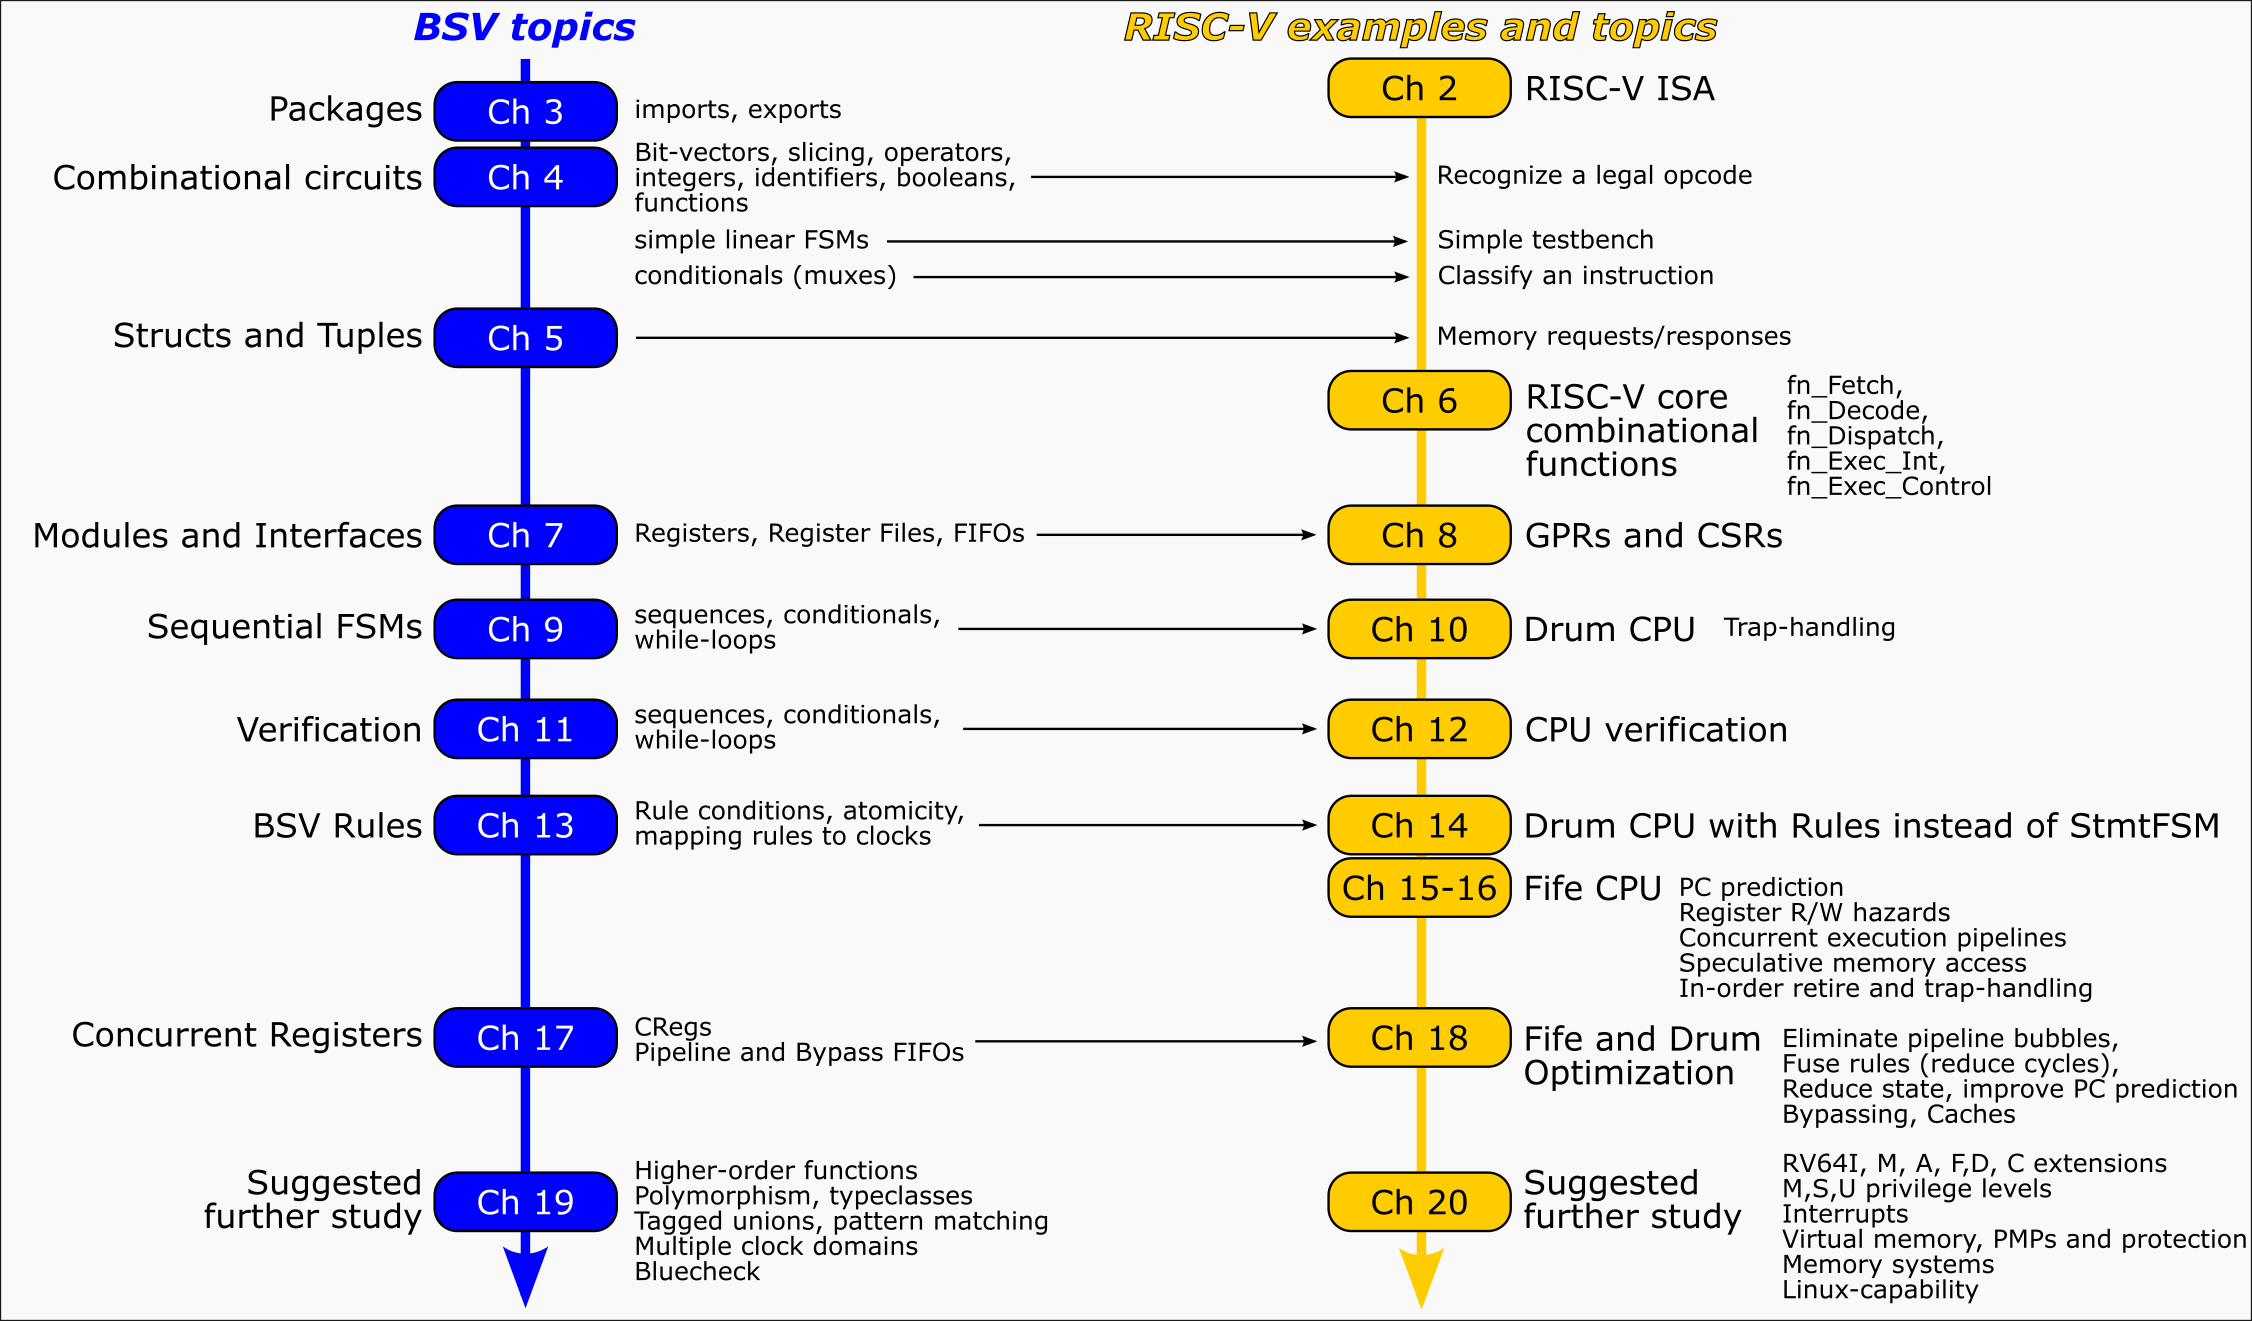
\includegraphics[height=0.825\textheight]{Fig_Chapter_Roadmap}}
\end{center}

\end{frame}

% ================================================================


% ================================================================

\begin{frame}
\frametitle{Flow of information between stages in Drum and Fife}

\label{Slide_Instr_Steps}

\footnotesize

\begin{center}
 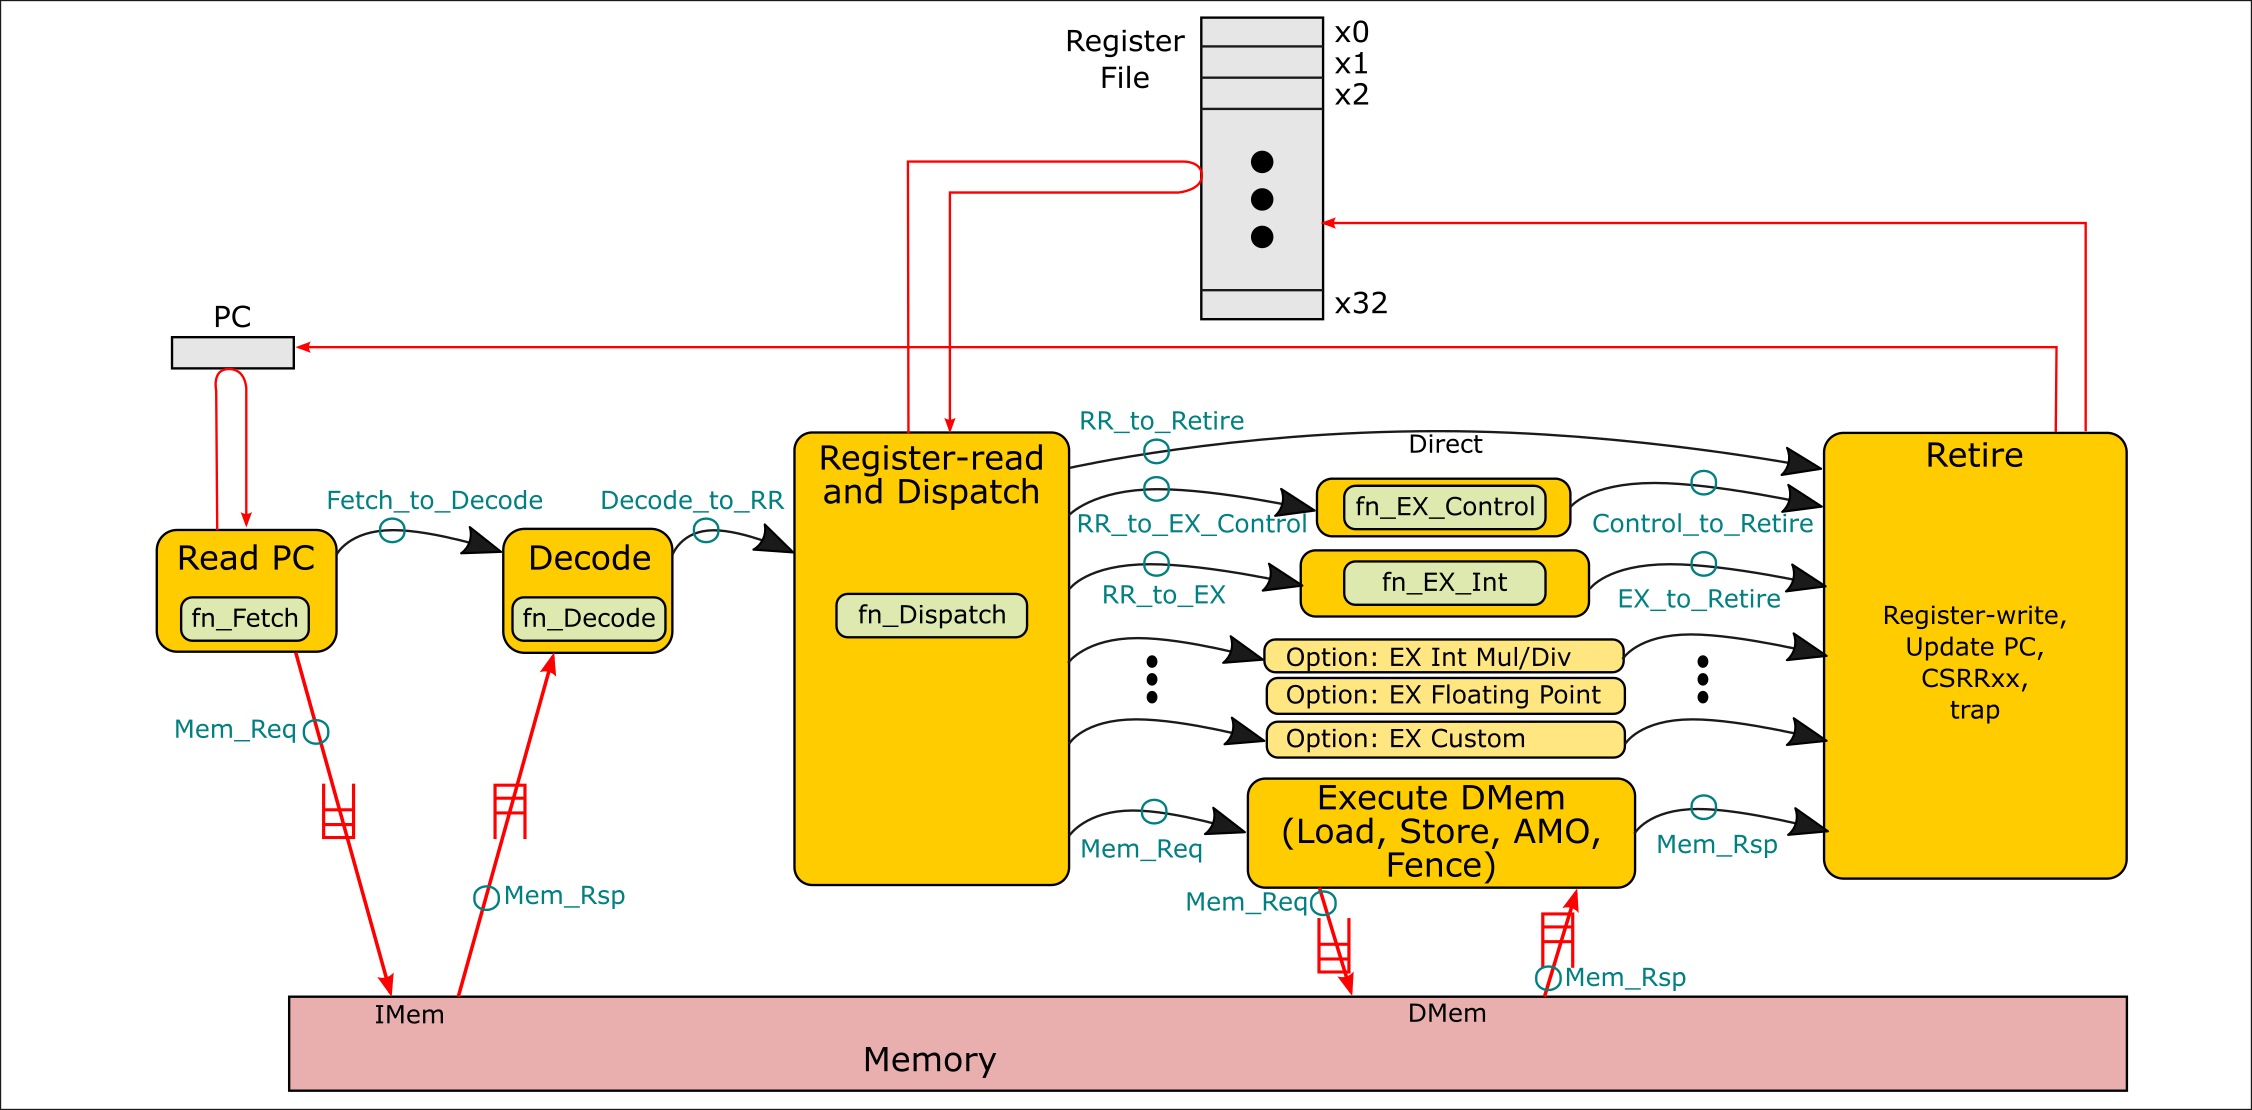
\includegraphics[height=0.6\textheight]{Fig_Instr_Exec_w_structs}
\end{center}

\end{frame}

% ================================================================

\begin{frame}
\frametitle{Table of Contents}

\tableofcontents

\end{frame}

% ****************************************************************

\section{Drum CPU: Module Interface (same for Drum and Fife)}

\begin{frame}

\begin{center}
  {\LARGE Drum CPU: Module Interface (same for Drum and Fife)}
\end{center}

\end{frame}

% ================================================================

\begin{frame}[fragile]
\frametitle{Drum CPU: Module Interface}

\footnotesize

\SHOWCODE{../Code_Extracts/CPU_IFC.tex}

\vspace{1ex}

The four FIFOs are for IMem and DMem requests (to memory) and IMem and DMem responses (from memory).

\vspace{2ex}

The {\tt init} method is used to set the starting PC value (and other initial values).

\vspace{1ex}

The {\tt set\_TIME} method is used to update the {\tt time} CSR.

\end{frame}

% ****************************************************************

\section{Drum CPU: Overall module structure and state}

\begin{frame}[fragile]

\begin{center}
  {\LARGE Drum CPU: Overall module structure and state}
\end{center}

\end{frame}

% ================================================================

\begin{frame}[fragile]
\frametitle{Drum CPU: Overall module structure}

\footnotesize

\begin{minipage}{0.725\textwidth}
\begin{Verbatim}[frame=single, label=From src\_Drum/CPU.bsv]
(* synthesize *)
module mkCPU (CPU_IFC);
   // ================================================================
   // STATE
   ...

   // ****************************************************************
   // BEHAVIOR
   ... help functions ...
   ... major actions  ...

   // ================================================================
   // BEHAVIOR: FSM or Rules

`include "Drum_FSM.bsv"

   // ****************************************************************
   // INTERFACE
   ...
endmodule
\end{Verbatim}
\end{minipage}
\hm
\emph{Details in slides that follow}

\end{frame}

% ================================================================

\begin{frame}[fragile]
\frametitle{Drum CPU: Module state (1/3)}

\footnotesize

\begin{minipage}{0.725\textwidth}
\begin{Verbatim}[frame=single, label=From src\_Drum/CPU.bsv]
   // Don't run until the PC (and other things) are initialized
   Reg #(Bool) rg_running <- mkReg (False);

   // For debugging in simulation only
   Reg #(File) rg_flog <- mkReg (InvalidFile);

   Reg #(Bit #(64)) rg_inum <- mkReg (0);    // For debugging only

   // The Program Counter
   Reg #(Bit #(XLEN)) rg_pc   <- mkReg (0);

   // General-Purpose Registers (GPRs)
   GPRs_IFC #(XLEN)  gprs <- mkGPRs_synth;

   // Control-and-Status Registers (CSRs)
   CSRs_IFC csrs <- mkCSRs;
\end{Verbatim}
\end{minipage}
\hm
\emph{... more ...}

\end{frame}

% ================================================================

\begin{frame}[fragile]
\frametitle{Drum CPU: Module state (2/3)}

\footnotesize

\begin{minipage}{0.725\textwidth}
\begin{Verbatim}[frame=single, label=From src\_Drum/CPU.bsv]
   // Inter-step registers
   Reg #(Fetch_to_Decode)      rg_Fetch_to_Decode      <- mkRegU;
   Reg #(Decode_to_RR)         rg_Decode_to_RR         <- mkRegU;
   Reg #(Result_Dispatch)      rg_Dispatch             <- mkRegU;
   Reg #(EX_Control_to_Retire) rg_EX_Control_to_Retire <- mkRegU;
   Reg #(EX_to_Retire)         rg_EX_to_Retire         <- mkRegU;

   // Regs to set up exception handling
   Reg #(Bool)        rg_exception <- mkReg (False);
   Reg #(Bit #(XLEN)) rg_epc       <- mkRegU;
   Reg #(Bit #(4))    rg_cause     <- mkRegU;
   Reg #(Bit #(XLEN)) rg_tval      <- mkRegU;
\end{Verbatim}
\end{minipage}
\hm
\emph{... more ...}

\vspace{2ex}

\begin{itemize}
 \item Inter-step registers hold intermediate values across clock cycles.

 \item Exception registers hold values across clocks until we perform
       the exception (in the final step).
\end{itemize}

\end{frame}

% ================================================================

\begin{frame}[fragile]
\frametitle{Drum CPU: Module state (3/3)}

\footnotesize

\begin{minipage}{0.725\textwidth}
\begin{Verbatim}[frame=single, label=From src\_Drum/CPU.bsv]
   // Paths to and from memory
   FIFOF #(Mem_Req) f_IMem_req  <- mkFIFOF;
   FIFOF #(Mem_Rsp) f_IMem_rsp  <- mkFIFOF;

   FIFOF #(Mem_Req) f_DMem_req  <- mkFIFOF;
   FIFOF #(Mem_Rsp) f_DMem_rsp  <- mkFIFOF;
\end{Verbatim}
\end{minipage}

\end{frame}

% ****************************************************************

\section{Drum CPU: some help functions}

\begin{frame}[fragile]

\begin{center}
  {\LARGE Drum CPU: Some help-functions}
\end{center}

\end{frame}

% ================================================================

\begin{frame}[fragile]
\frametitle{Drum CPU: Some help-functions (1/3)}

\footnotesize

(Help-functions just encapsulate a few actions that are repeated in several places.)

\vspace{5ex}

This function writes a result of an instruction (a value) into the {\tt rd} register:

\vspace{4ex}

\begin{minipage}{0.725\textwidth}
\SHOWCODE{../Code_Extracts/Drum_upd_rd.tex}
\end{minipage}

\end{frame}

% ================================================================

\begin{frame}[fragile]
\frametitle{Drum CPU: Some help-functions (2/3)}

\footnotesize

(Help-functions just encapsulate a few actions that are repeated in several places.)

\vspace{5ex}

This function increments the PC and the instruction-number, as we retire each instruction:

\vspace{4ex}

\begin{minipage}{0.725\textwidth}
\SHOWCODE{../Code_Extracts/Drum_redirect.tex}
\end{minipage}

\end{frame}

% ================================================================

\begin{frame}[fragile]
\frametitle{Drum CPU: Some help-functions (3/3)}

\footnotesize

(Help-functions just encapsulate a few actions that are repeated in several places.)

\vspace{5ex}

This function records information for later trap-handling:

\vspace{4ex}

\begin{minipage}{0.725\textwidth}
\SHOWCODE{../Code_Extracts/Drum_setup_exc.tex}
\end{minipage}

\end{frame}

% ****************************************************************

\section{Drum CPU: top-level FSM}

\begin{frame}[fragile]

\begin{center}
  {\LARGE Drum CPU: top-level FSM}
\end{center}

\end{frame}

% ================================================================

\begin{frame}[fragile]
\frametitle{Drum CPU: top-level FSM (1/2)}

\footnotesize

\begin{minipage}{0.725\textwidth}
 \SHOWCODE{../Code_Extracts/Drum_FSM.tex}
\end{minipage}

\vspace{5ex}

The very top-level is very simple and self-evident.

\vspace{2ex}

The {\tt await} statement waits until the {\tt init} method has set
the initial PC, so that we start fetching from the correct address.

\end{frame}

% ================================================================

\begin{frame}[fragile]
\frametitle{Drum CPU: top-level FSM (2/2)}

\footnotesize

\begin{minipage}{0.5\textwidth}
 \SHOWCODETINY{../Code_Extracts/Drum_exec_one_instr.tex}
\end{minipage}
\hm
\begin{minipage}{0.45\textwidth}
 This is practically a direct coding of the instruction-execution steps
 in the diagram on Slide~\ref{Slide_Instr_Steps}.
\end{minipage}


\end{frame}

% ****************************************************************

\section{Drum CPU: FSM Fetch step}

\begin{frame}[fragile]
\frametitle{Drum CPU: FSM Fetch step}

\footnotesize

\begin{minipage}{0.75\textwidth}
 \SHOWCODE{../Code_Extracts/Drum_Fetch.tex}
\end{minipage}
\hm
\begin{minipage}{0.2\textwidth}
 Just invokes {\tt fn\_Fetch} and sends the two results into a register for Fetch and
 into a FIFO for IMem memory.
\end{minipage}

\end{frame}

% ****************************************************************

\section{Drum CPU: FSM Decode step}

\begin{frame}[fragile]
\frametitle{Drum CPU: FSM Decode step}

\footnotesize

\begin{minipage}{0.75\textwidth}
 \SHOWCODE{../Code_Extracts/Drum_Decode.tex}
\end{minipage}
\hm
\begin{minipage}{0.2\textwidth}
 Just invokes {\tt fn\_Decode} on the inputs from Fetch and memory,
 and sends the result into a register for Register-Read-and-Dispatch.
\end{minipage}

\end{frame}

% ****************************************************************

\section{Drum CPU: FSM Register-Read and Dispatch step}

\begin{frame}[fragile]
\frametitle{Drum CPU: FSM Register-Read and Dispatch step}

\footnotesize

\begin{minipage}{0.75\textwidth}
 \SHOWCODE{../Code_Extracts/Drum_RRD.tex}
\end{minipage}
\hm
\begin{minipage}{0.2\textwidth}
 Using input from Decode, reads two registers {\tt rs1} and {\tt rs2};
 then invokes {\tt fn\_Dispatch}, and
 and sends the result into a register for the Execute stage.
\end{minipage}

\end{frame}

% ****************************************************************

\section{Drum CPU: FSM Execute and Retire step}

\begin{frame}[fragile]

\begin{center}
  {\LARGE Drum CPU: FSM Execute and Retire step}
\end{center}

\end{frame}

% ================================================================

\begin{frame}[fragile]
\frametitle{Drum CPU: FSM Execute and Retire step flows}

\begin{minipage}{0.75\textwidth}
 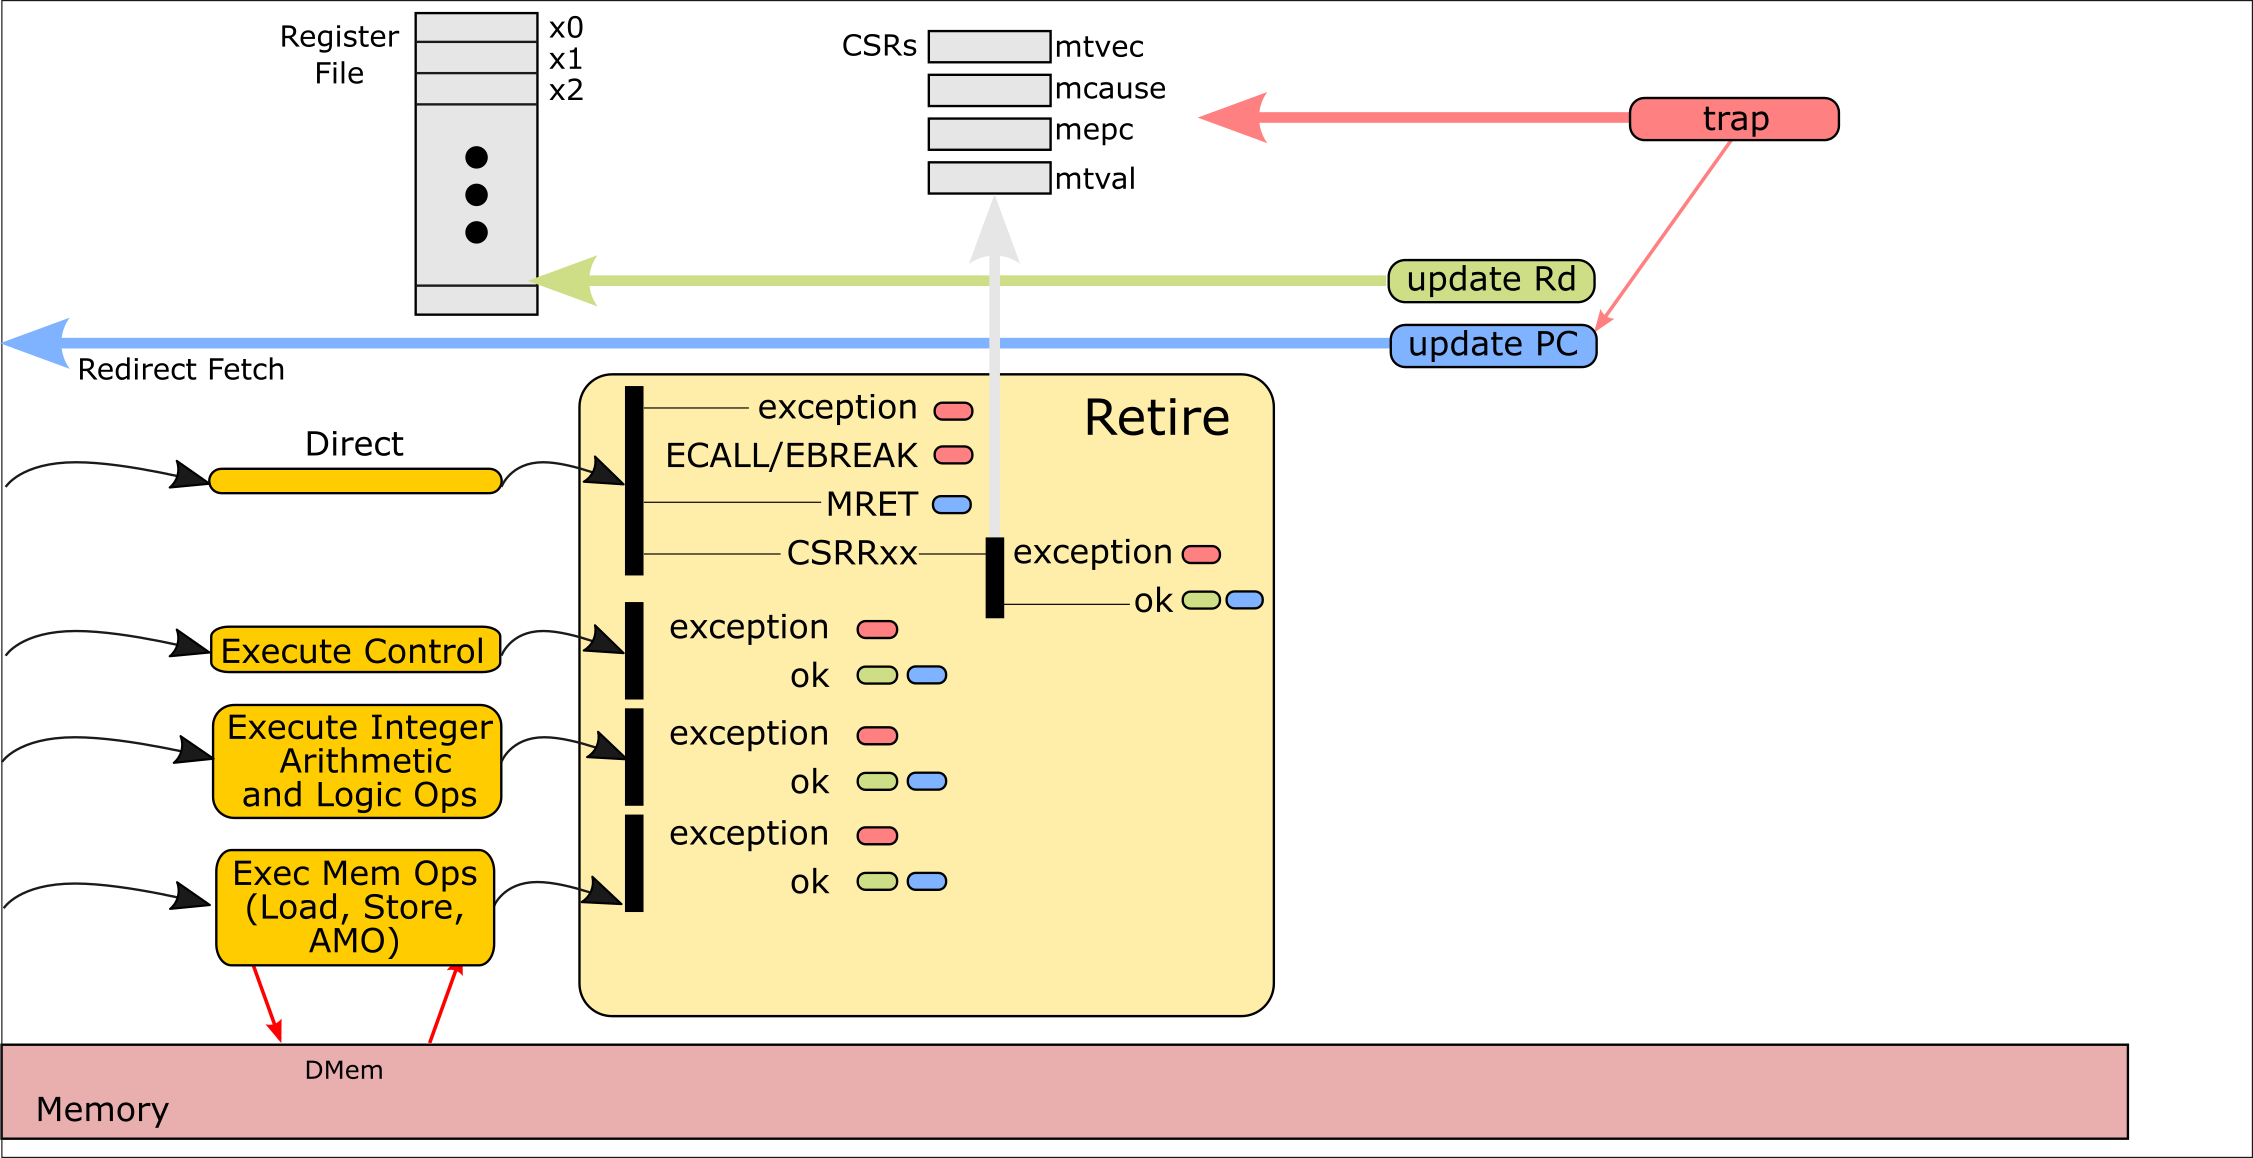
\includegraphics[width=\textwidth]{Fig_Retire_Layers_1}
\end{minipage}
\hm
\begin{minipage}{0.2\textwidth}
4 possible flows.
\begin{itemize}
 \item Direct
 \item Control
 \item Int
 \item DMem
\end{itemize}

\vspace{2ex}

Each ultimately resulting in up to 3 possible actions.
\end{minipage}

\end{frame}

% ================================================================

\begin{frame}[fragile]
\frametitle{Drum CPU: Updating the {\tt minstret} CSR (counting instructions retired)}

\footnotesize

The {\tt minstret} CSR is incremented for each instruction retired.

\emph{Except:}

\begin{itemize}

 \item An instruction that raises an exception.

 \item A CSRRxx instruction that writes a value into {\tt minstret}.

\end{itemize}

\vspace{2ex}

We increment using:
\begin{tabbing}\tt
\hmm  csrs.ma\_incr\_instret;
\end{tabbing}

\vspace{2ex}

The {\tt minstret} and {\tt mcycle} CSRs are useful in performance
measurement (instructions/cycle).

\end{frame}

% ================================================================

\begin{frame}[fragile]
\frametitle{Drum CPU: Execute and Retire Direct flow (1/4)}

\footnotesize

\begin{minipage}{0.725\textwidth}
\begin{Verbatim}[frame=single, label=From src\_Drum/CPU.bsv]
   Action a_Retire_direct =
   action
      let x_direct = rg_Dispatch.to_Retire;
      if (x_direct.exception) begin
	 fa_setup_exception (x_direct.pc,        // epc
			     x_direct.cause,     // cause
			     x_direct.tval);     // tval
	 log_Retire_Direct_exc (rg_flog, x_direct);
      end
      // ----------------
      ...
\end{Verbatim}
\end{minipage}

\end{frame}

% ================================================================

\begin{frame}[fragile]
\frametitle{Drum CPU: Execute and Retire Direct flow (2/4)}

\footnotesize

\begin{minipage}{0.725\textwidth}
\begin{Verbatim}[frame=single, label=From src\_Drum/CPU.bsv]
      ...
      // ----------------
      else if (is_legal_CSRRxx (x_direct.instr)) begin
	 match { .exc, .rd_val } <- csrs.mav_csrrxx (x_direct.instr,
						     x_direct.rs1_val);
	 if (exc)
	    fa_setup_exception (x_direct.pc,                  // epc
				cause_ILLEGAL_INSTRUCTION,    // cause
				x_direct.instr);              // tval
	 else begin
	    fa_update_rd (x_direct, rd_val);
	    fa_redirect_Fetch (x_direct.fallthru_pc);
	 end
	 log_Retire_CSRRxx (rg_flog, exc, x_direct);
      end
      // ----------------
      ...
\end{Verbatim}
\end{minipage}

\end{frame}

% ================================================================

\begin{frame}[fragile]
\frametitle{Drum CPU: Execute and Retire Direct flow (3/4)}

\footnotesize

\begin{minipage}{0.725\textwidth}
\begin{Verbatim}[frame=single, label=From src\_Drum/CPU.bsv]
      ...
      // ----------------
      else if (is_legal_MRET (x_direct.instr)) begin
	 fa_redirect_Fetch (csrs.read_epc);
	 csrs.ma_incr_instret;
	 log_Retire_MRET (rg_flog, x_direct);
      end
      // ----------------
      ...
\end{Verbatim}
\end{minipage}

\end{frame}

% ================================================================

\begin{frame}[fragile]
\frametitle{Drum CPU: Execute and Retire Direct flow (4/4)}

\footnotesize

\begin{minipage}{0.725\textwidth}
\begin{Verbatim}[frame=single, label=From src\_Drum/CPU.bsv]
      ...
      // ----------------
      else if (is_legal_ECALL (x_direct.instr)
	       || is_legal_EBREAK (x_direct.instr))
	 begin
	    let cause = ((x_direct.instr [20] == 0)
			 ? cause_ECALL_FROM_M
			 : cause_BREAKPOINT);
	    fa_setup_exception (x_direct.pc,    // epc
				cause,
				0);             // tval
	    csrs.ma_incr_instret;
	    log_Retire_ECALL_EBREAK (rg_flog, x_direct);
	 end
      else begin
	 wr_log2 (rg_flog, $format ("CPU.EX.Direct: IMPOSSIBLE"));
	 $finish (1);
      end
   endaction;
\end{Verbatim}
\end{minipage}

\end{frame}

% ================================================================

\begin{frame}[fragile]
\frametitle{Drum CPU: Execute and Retire Control flow}

\footnotesize

\begin{minipage}{0.725\textwidth}
\begin{Verbatim}[frame=single, label=From src\_Drum/CPU.bsv]
   Action a_EX_Control =
   action
      let x = rg_Dispatch.to_EX_Control;
      let y <- fn_EX_Control (x, rg_flog);
      rg_EX_Control_to_Retire <= y;
      ...
   endaction;
\end{Verbatim}
\end{minipage}

\begin{minipage}{0.725\textwidth}
\begin{Verbatim}[frame=single]
   Action a_Retire_Control =
   action
      let x_direct  = rg_Dispatch.to_Retire;
      let x_control = rg_EX_Control_to_Retire;
      if (x_control.exception)
	 fa_setup_exception (x_direct.pc,
			     x_control.cause,
			     x_control.tval);
      else begin
	 fa_update_rd (x_direct, x_control.data);
	 fa_redirect_Fetch (x_control.next_pc);
	 csrs.ma_incr_instret;
      end
      ...
   endaction;
\end{Verbatim}
\end{minipage}

\end{frame}

% ================================================================

\begin{frame}[fragile]
\frametitle{Drum CPU: Execute and Retire Int flow}

\footnotesize

\begin{minipage}{0.725\textwidth}
\begin{Verbatim}[frame=single, label=From src\_Drum/CPU.bsv]
   Action a_EX_Int =
   action
      let x = rg_Dispatch.to_EX;
      let y <- fn_EX_Int (x, rg_flog);
      rg_EX_to_Retire <= y;
      ...
   endaction;
\end{Verbatim}
\end{minipage}

\begin{minipage}{0.725\textwidth}
\begin{Verbatim}[frame=single]
   Action a_Retire_Int =
   action
      if (rg_EX_to_Retire.exception)
	 fa_setup_exception (rg_Dispatch.to_Retire.pc,
			     rg_EX_to_Retire.cause,
			     rg_EX_to_Retire.tval);
      else begin
	 fa_update_rd (rg_Dispatch.to_Retire, rg_EX_to_Retire.data);
	 fa_redirect_Fetch (rg_Dispatch.to_Retire.fallthru_pc);
	 csrs.ma_incr_instret;
      end
      ...
   endaction;
\end{Verbatim}
\end{minipage}

\end{frame}

% ================================================================

\begin{frame}[fragile]
\frametitle{Drum CPU: Execute and Retire DMem flow (1/2)}

\footnotesize

\begin{minipage}{0.725\textwidth}
\begin{Verbatim}[frame=single, label=From src\_Drum/CPU.bsv]
   Action a_EX_DMem =
   action
      Mem_Req y = rg_Dispatch.to_EX_DMem;
      f_DMem_req.enq (y);
      ...
   endaction;
\end{Verbatim}
\end{minipage}

\end{frame}

% ================================================================

\begin{frame}[fragile]
\frametitle{Drum CPU: Execute and Retire DMem flow (2/2)}

\footnotesize

\begin{minipage}{0.725\textwidth}\scriptsize
\begin{Verbatim}[frame=single, label=From src\_Drum/CPU.bsv]
   Action a_Retire_DMem =
   action
      let x_direct = rg_Dispatch.to_Retire;
      let mem_rsp <- pop_o (to_FIFOF_O (f_DMem_rsp));
      Bool exception = ((mem_rsp.rsp_type == MEM_RSP_ERR)
			|| (mem_rsp.rsp_type == MEM_RSP_MISALIGNED));
      if (exception) begin
	 Bit #(4) cause = ((mem_rsp.rsp_type == MEM_RSP_MISALIGNED)
			   ? (is_LOAD (x_direct.instr)
			      ? cause_LOAD_ADDRESS_MISALIGNED
			      : cause_STORE_AMO_ADDRESS_MISALIGNED)
			   : (is_LOAD (x_direct.instr)
			      ? cause_LOAD_ACCESS_FAULT
			      : cause_STORE_AMO_ACCESS_FAULT));
	 fa_setup_exception (x_direct.pc,                 // epc
			     cause,
			     truncate (mem_rsp.addr));    // tval
      end
      else begin
	 fa_update_rd (x_direct, truncate (mem_rsp.data));
	 fa_redirect_Fetch (x_direct.fallthru_pc);
	 csrs.ma_incr_instret;
      end
      ...
   endaction;
\end{Verbatim}
\end{minipage}

\end{frame}

% ================================================================

\begin{frame}[fragile]
\frametitle{Drum CPU: action for exceptions}

\footnotesize

\begin{minipage}{0.725\textwidth}
\begin{Verbatim}[frame=single, label=From src\_Drum/CPU.bsv]
   Action a_exception =
   action
      Bool is_interrupt = False;
      Bit #(XLEN) tvec_pc <- csrs.mav_exception (rg_epc,
						 is_interrupt,
						 rg_cause,
						 rg_tval);
      rg_exception <= False;
      fa_redirect_Fetch (tvec_pc);
      ...
   endaction;
\end{Verbatim}
\end{minipage}

\end{frame}

% ****************************************************************

\section{Drum CPU: Final Comments}

\begin{frame}[fragile]
\frametitle{{\BSV}: {\tt StmtFSM} final comments}

\footnotesize

Drum CPU code, using {\tt StmtFSM}, looks just like a C/C++ program
with somewhat different syntax.

\vspace{2ex}

So: can't we just code it in C/C++ and compile that to hardware?

\vspace{2ex}

\begin{itemize}
        
 \item Difficult to compile \emph{general-purpose} C into hardware.

       C has many constructs that have no obvious mapping into
       hardware, such as pointers, the address-of operator ``\&'',
       address arithmetic, malloc, and so on.

       But can’t we define a restricted subset of C suitable for
       hardware design?

       Compilation is still very difficult: no distinction between
       variables used to hold state (registers) {\vs} variables used
       to hold temporary intermediate values (wires); no distinction
       between pure and side-effect constructs; ...

 \item No concurrency.  It may be possible to compile a subset of C to
       hardware, similar to Drum.  But this is the easy case
       (completely sequential).  Very hard to generalize to pipelines
       and more concurrent implementations (Fife, and beyond).

\end{itemize}

\end{frame}

% ****************************************************************

% -*- mode: fundamental -*-

% Slides accompanying "Learn RISC-V CPU Implementation and BSV" book
% Copyright (c) 2024 Rishiyur S. Nikhil, All Rights Reserved

% This is a postamble shared by all the slide decks

% ================================================================

\begin{frame}

\begin{center}
  {\LARGE End}
\end{center}

\end{frame}

% ================================================================


% ****************************************************************

\end{document}
% ****************************************************************
